% buaa基于ctexbook模板
% 模板选项:
%======================
% I.论文类型(thesis)
%--------------------
% a.学术硕士论文(master)[缺省值]
% b.专业硕士论文(professional)
% c.博士论文(doctor)
%--------------------
% II.密级(permission)
%--------------------
% a.公开(public)[缺省值]
% b.内部(privacy)
% c.秘密(secret=secret3)
% c.1.秘密3年(secret3)
% c.2.秘密5年(secret5)
% c.3.秘密10年(secret10)
% c.4.秘密永久(secret*)
% d.机密(classified=classified5)
% d.1.机密3年(classified3)
% d.2.机密5年(classified5)
% d.3.机密10年(classified10)
% d.4.机密永久(classified*)
% e.绝密(topsecret=topsecret10)
% e.1.绝密3年(topsecret3)
% e.2.绝密5年(topsecret5)
% e.3.绝密10年(topsecret10)
% e.4.绝密永久(topsecret*)
%--------------------
% III.打印设置(printtype)
%--------------------
% a.单面打印(oneside)[缺省值]
% b.双面打印(twoside)
%--------------------
% IV.系统类型(ostype)
%--------------------
% a.win(oneside)[缺省值]
% b.linux (linux)
% c.mac (mac)
%--------------------
% V.ctexbook设置选项(<ctexbookoptions>)
%--------------------
% ...
%======================
% 其他说明:
% 1. Mac系统请使用mac选项,并使用XeLaTeX编译。
% 2. 可加入额外ctexbook文档类的选项,其将会被传递给ctexbook。
%    例如:\documentclass[fontset=founder]{buaa}
% 3. CTeX在Linux下默认使用Fandol字体,为避免某些生僻字无法显示,在系统已安装方正
%    字体的前提下可通过fontset=founder选项常用方正字体。
%=================================================================
% buaa模板已内嵌以下LaTeX工具包:
%--------------------
% ifthen, etoolbox, titletoc, remreset,
% geometry, fancyhdr, setspace,
% float, graphicx, subfigure, epstopdf,
% array, enumitem,
% booktabs, longtable, multirow, caption,
% listings, algorithm2e, amsmath, amsthm,
% hyperref, pifont, color, soul,
% ---
% For Win: times
% For Lin: newtxtext, newtxmath
% For Mac: times, fontspec
%--------------------
% 请在此处添加额外工具包>>
%=================================================================
% buaa模板已内嵌以下LaTeX宏:
%--------------------
% \highlight{text} % 黄色高亮
%--------------------
% 请在此处添加自定义宏>>
%%=================================================================

\documentclass[master,public,twoside,win,AutoFakeBold]{buaa}
\usepackage{tabularray}
\UseTblrLibrary{siunitx}
\usepackage{multirow}
\usepackage{hyperref}
\usepackage[usenames,dvipsnames,svgnames,table]{xcolor}
\usepackage{pdfpages}

\usepackage{listings}
\lstset{
  basicstyle=\ttfamily\small,
  commentstyle=\ttfamily,
  linewidth=\linewidth,
  frame=single,
  showstringspaces=false,
  columns=flexible,
  language=C,
  breaklines=true,
  mathescape,
  escapeinside=||
}
\let\origthelstnumber\thelstnumber
\makeatletter
\newcommand*\Suppressnumber{%
  \lst@AddToHook{OnNewLine}{%
    \let\thelstnumber\relax%
     \advance\c@lstnumber-\@ne\relax%
    }%
}

\newcommand*\Reactivatenumber{%
  \lst@AddToHook{OnNewLine}{%
   \let\thelstnumber\origthelstnumber%
   \advance\c@lstnumber\@ne\relax}%
}
\makeatother

%=================================================================
% 开启/关闭引用编号颜色:参考文献,公式,图,表,算法 等……
\refcolor{on}   % 开启: on[默认]; 关闭: off;

% 摘要和正文从右侧页开始,单面打印请关闭
\beginright{on} % 开启: on; 关闭: off[默认];

%盲评模式,开启后不显示学校等信息 ,注意自行修改致谢和学术成果
\blindmode{off}   % 开启: on; 关闭: off[默认];

% 图标目录
\Listfigtab{bi} % 启用: on[默认]; 双标题:bi; 关闭: off;

% 空白页留字
\emptypagewords{[ -- This page is a preset empty page -- ]}

% 不显示超链接方框
% \hypersetup{hidelinks}

%=================================================================
% 论文题目及副标题-{中文}{英文}
\Title{机动战士驾驶}{Mobile Suit Driving}
%\Subtitle{学位论文~\LaTeX{}模板}

% 申请学位级别
\Branch{ }
% 研究方向
\Field{ }

% 院系,专业及研究方向
\Department{机动战士驾驶}

% 博士+学硕配置------------>
% 一级学科/学科专业
\Major{人机神经链接}
% 二级学科
\Majorsec{}
% 学科专业
\MasterMajor{}

% 专硕配置------------>
%研究方向
\ProCategory{ }
\ProField{ }
\ProName{ }

% 导师信息-{中文名}{英文名}{职称}
\Tutor{李四}{LI Si}{教授}
%\Cotutor{副导师姓名}{Cotutor}{高工}

% 学生姓名-{中文名}{英文名}
\Author{张三}{ZHANG Sang}
% 论文编号
\StudentID{}

% 中图分类号
\CLC{}

% 时间节点-{月}{日}{年}
%入学时间
\DateEnroll{00}{00}{0000}
%毕业时间
\DateGraduate{00}{00}{0000}
%论文提交日期
\DateSubmit{00}{00}{0000}
%论文答辩日期
\DateDefence{00}{00}{0000}

%%=================================================================
% 摘要-{中文}{英文}
\Abstract{%
  中文摘要。
  }{%
  English abstract. 
}
% 关键字-{中文}{英文}
\Keyword{%
    关键词
  }{%
    keyword
}


\begin{document}

% 绪论
\chapter{绪论}

\section{概述}
学位论文是标明作者从事科学研究取得的创造性成果和创新见解,并以此为内容撰写的、作为申请学位时评审用的学术论文。

硕士学位论文应表明作者在本门学科上掌握了坚实的基础理论和系统的专门知识,对所研究的课题有新的见解,并具有从事科学研究工作或独立担负专门技术工作能力。

博士学位论文应表明作者在本门学科上掌握了坚实宽广的基础理论和系统深入的专门知识,在科学和专门技术上做出了创造性的成果,并具有独立从事科学研究工作的能力。

为提高研究生学位论文的质量,做到学位论文在内容和格式上的统一和规范,根据《中华人民共和国国家标准科学技术报告、学位论文和学术论文的编写格式》(GB/T 7713.1—2006)的规定,特制定《安徽大学研究生撰写学位论文的规定》。

\section{论文的基本要求}
论文应立论正确、推理严谨、说明透彻、数据可靠。

论文应结构合理、层次分明、叙述准确、文字简练、文图规范。对于涉及作者创新性工作和研究特点的内容应重点论述,做到数据或实例丰富、分析全面深入。文中引用的文献资料必须注明来源,使用的计量单位、绘图规范应符合国家标准。

论文的学术水平应满足《安徽大学申请博士、硕士学位学术成果基本要求》的要求。

\section{论文内容}
包括:选题的背景、依据及意义;文献及相关研究综述、研究及设计方案、试验方法、装置和试验结果;理论的证明、分析和结论;重要的计算、数据、图表、曲线及相关分析;必要的附录、相关的参考文献目录等。

对于合作完成的项目,论文的内容应侧重本人的研究工作。论文中有关与指导教师或他人共同研究、试验的部分以及引用他人研究成果的部分都要明确说明。

学位论文一般应由12个部分组成,见表\ref{tab:papercomponents}:
\begin{table}[h]
    \caption{学位论文组成}
    \label{tab:papercomponents}
    \centering
    \begin{tabular}{cp{16\ccwd}p{4cm}}
      \toprule
      {\bfseries 装订顺序} & \multicolumn{1}{c} {\bfseries 内容} & \multicolumn{1}{c} {\bfseries 说明}  \\
      \midrule
      1 & 封面(中、英文)& \\
      2 & 题名页          & \\
      3 & 独创性声明和使用授权书 & \\
      4 & 中文摘要        & \\
      5 & 英文摘要        & \\
      6 & 目录            & \\
      7 & 图表清单及主要符号表  & 根据具体情况可省略 \\
      8 & 主体部分        & \\
      9 & 参考文献        & \\
      10& 附录            & \\
      11&攻读博士学位期间取得的研究成果/攻读硕士学位期间取得的学术成果 & 注意博士的是研究成果,硕士的是学术成果 \\
      12& 致谢            & \\
      \bottomrule
    \end{tabular}
  \end{table}

\section{论文每部分内容的具体要求}

\subsection{论文的封面}

{\bfseries 封皮:}  由各研究生培养单位到研究生院学位办领取。

{\bfseries 中图分类号:} 根据论文的主题内容对照《中国图书馆分类法》选取(到本校图书馆网站上可查)。

{\bfseries 论文编号:} 为“我校单位代码(10357)+ 学号”,如:“10357H19101001”。

{\bfseries 密级:} 保密论文须直接注明密级及相应的保密期限,如系公开论文此项不注。

{\bfseries 论文题目:} 应准确、鲜明、简洁,能概括整个论文中最主要和最重要的内容。论文题目中所用到的词应考虑到为检索提供特定实用的信息(如关键词),一般不宜超过25个中文字,若语意未尽,可用副标题补充说明。副标题应处于从属地位,一般可在题目的下一行用破折号“——”引出。论文题目应避免使用不常用缩略词、首字母缩写字、字符、代号和公式等。

{\bfseries 学科专业:} 以国务院学位委员会批准的授予博士、硕士学位和培养研究生的学科、专业目录中的学科专业为准。对专业学位应填写相应的专业学位名称(如工商管理硕士)或工程领域(如生物工程)。

{\bfseries 指导教师:} 指导教师的署名应以研究生院批准招生的为准,学术学位论文一般只能写一名指导教师,如有经主管部门批准的副指导教师或联合指导教师,可增1名指导教师。专业学位论文需写2名指导教师,分别为校内、企业(研究院所)导师,导师组指导可再增1名校内指导教师。

\subsection{提名页}
提名页是对学位论文进行著录的依据,内容包括封面并比封面内容更为详细。

{\bfseries 研究方向:} 只填写一个,应比学科专业的二级学科更具体,但比论文关键词的覆盖面更广,一般为学科分类号对应的研究方向。

{\bfseries 学科分类号:} 按照《学科分类与代码》(GB/T 13745)(可以空,由论文保管部门填写)。

{\bfseries 申请学位级别:} 指按《中华人民共和国学位条例暂行实施办法》规定的名称进行申请的学位级别,填写“学科门类+学位”,学科门类有哲学、经济学、法学、教育学、文学、历史学、理学、工学、农学、医学、军事学、管理学和艺术学等13个学科门类以及专业学位类别(如工程、工商管理、公共管理、软件工程),如:工学硕士、文学硕士、工程硕士、工商管理硕士、公共管理硕士、软件工程硕士、工学博士、管理学博士和理学博士等。

{\bfseries 工作完成时间:} 包括学习时间(从研究生入学至毕业的时间段)、论文提交日期(论文送审评阅时间)、论文答辩日期、学位授予日期;除学位授予日期可以不填外,其它均需准确填写,一律用阿拉伯数字填写日期。、

\subsection{独创性声明和使用授权书}
学位论文的独创性声明和使用授权书的内容和格式见附件10,必须由作者、指导教师亲笔签名并填写日期。

\subsection{摘要}
中文摘要内容包括: “摘要”字样,摘要正文,关键词。对于中英文摘要,都必须在摘要的最下方另起一行,用显著的字符注明本文的关键词。

摘要是学位论文内容的简短陈述,应体现论文工作的核心思想。论文摘要应力求语言精练准确,博士学位论文的中文摘要一般约800~1200字;硕士学位论文的中文摘要一般约500字。摘要内容应涉及本项科研工作的目的和意义、研究思想和方法、研究成果和结论,博士学位论文必须突出论文的创造性成果,硕士学位论文必须突出论文的新见解。
关键词:是为用户查找文献,从文中选取出来用来揭示全文主题内容的一组词语或术语,应尽量采用词表中的规范词(参照相应的技术术语标准)。关键词一般为3~5个,按词条的外延层次排列(外延大的排在前面)。关键词之间用逗号分开,最后一个关键词后不打标点符号。
英文摘要:为了国际交流的需要,论文须有英文摘要。英文摘要的内容及关键词应与中文摘要及关键词一致,要符合英语语法,语句通顺,文字流畅。英文和汉语拼音一律为Times New Roman体,字号与中文摘要相同。

\subsection{目录}
目录按章、节、条序号和标题编写,一般为二级或三级,目录中应包括绪论(或引言)、论文主体、结论、附录、参考文献、附录、攻读学位期间取得的成果等。

\subsection{图表清单及主要符号表}
如果论文中图表较多,可以分别列出清单置于目录之后。图的清单应有序号、图题和页码。表的清单应有序号、表题和页码。

全文中常用的符号、标志、缩略词、首字母缩写、计量单位、名词、术语等的注释说明,如需汇集,可集中在图和表清单后的主要符号表中列出,符号表排列顺序按英文及其它相关文字顺序排出。

\subsection{主体部分}
论文主体一般应包括:绪论(或引言)、正文、结论等部分。

\subsubsection{章节标题及层次}
论文主体分章节撰写, 每章应另起一页。

章节标题要突出重点、简明扼要、层次清晰。字数一般在15字以内, 不得使用标点符号。标题中尽量不采用英文缩写词,对必须采用者,应使用本行业的通用缩写词。

层次以少为宜,根据实际需要选择。三级标题的层次对理工类建议按章(如“第一章” )、节(如“1.1” )、条(如“1.1.1” )的格式编写;对社科、文学类建议按章(如“一、” )、节(如“ (一)” )、条(如“ 1、” )的格式编写,各章题序的阿拉伯数字用Times New Roman体。

\subsubsection{绪论}
绪论(或引言)一般作为第一章,是论文主体的开端。绪论的内容应简要说明研究工作的目的、范围、相关领域的前人工作和知识空白、理论基础、研究设想、研究方法和实验设计、预期结果和意义等。应言简意赅,不要与摘要雷同,不要写成摘要的注释。一般教科书中有的知识,在绪论中不必赘述。

学位论文为了反映出作者确已掌握了坚实的基础理论和系统的专门知识,具有开阔的科学视野,对研究方案作了充分论证,因此,有关历史回顾和前人工作的综述分析,以及理论分析等,可以单独成章,用足够的文字叙述。博士学位论文绪论一般不少于0.8万字,硕士学位论文绪论一般不少于0.5 万字。

\subsubsection{正文}
正文是学位论文的核心部分,占主要篇幅。

由于研究工作涉及的学科、选题、研究方法、工作进程、结果表达方式的不同,正文可以包括如下相关内容:调查对象、实验和观测方法、仪器设备、材料原料、实验和观测结果、计算方法和编程原理、数据资料、经过加工整理的图表、形成的论点和导出的结论等。总之,作者应根据研究工作的内容,阐明研究方案和实验方法,突出自己的创新性和特色工作,做到论点明确、论据充分、结论可信,与同类和相关工作的比较分析清楚。

正文应该结构合理,层次分明,推理严密,文笔流畅,内容集中简练,图表、参考文献规范。博士学位论文一般为6-10万字,硕士学位论文一般为3-5万字。

\subsubsection{结论}
学位论文的结论单独作为一章,但不加章号。

结论是整篇学位论文的总结,是整篇论文的归宿,不是正文中各章节的小结的简单重复。要求精炼、准确、完整地阐述自己的创造性工作或新的见解及其意义和作用。在结论或讨论中可提出尚待解决的问题,进一步研究的设想,仪器设备的改进以及其它与论文工作有关的建议等。

如果不可能导出应有的结论,也可以没有结论而进行必要的讨论。

\subsection{参考文献}
学术研究应精确、有据、坦诚、创新和积累。而其中精确、有据和积累需要建立在正确对待前人学术成果的基础上。对学位论文中包含的其他人已经发表或撰写过的材料,或为获得其它教育机构的学位证书而使用过的材料,或与作者一同工作的指导教师和同事对本研究所做的任何贡献,均应在论文中做出明确的标引和说明。

因此,凡有直接引用他人成果(文字、数字、事实以及转述他人的观点)之处,均应加标注说明列于参考文献中,以避免论文抄袭现象的发生。研究生学位论文参考文献著录及标引按照国家标准《文后参考文献著录规则》(GB7714)和中国博硕士学位论文编写与交换格式。

\subsection{附录}
附录是作为论文主体的补充项目,并不是必需的。下列内容可以作为附录编于论文后:
\begin{enumerate}
    \item [(1)] 为了整篇论文材料的完整,但编入正文又有损于编排的条理和逻辑性,这一材料包括比正文更为详尽的信息、研究方法和技术更深入的叙述,建议可以阅读的参考文献题录,对了解正文内容有用的补充信息等。
    \item [(2)] 由于篇幅过大或取材于复制品而不便于编入正文的材料。
    \item [(3)] 不便于编入正文的罕见的珍贵资料或需要特别保密的技术细节和详细方案(这种情况可单列成册)。
    \item [(4)] 对一般读者并非必要阅读,但对本专业同行有参考价值的资料。
    \item [(5)] 某些重要的原始数据、过长的数学推导、计算程序、框图、结构图、注释、统计表、计算机打印输出文件等。
\end{enumerate}

\subsection{攻读博士学位期间取得的研究成果/攻读硕士学位期间取得的学术成果}
对于博士学位论文,本条目名称用“攻读博士学位期间取得的研究成果”,一般包括以下两项内容:

攻读博士学位期间取得的学术成果:列出攻读博士学位期间发表(含录用)的与学位论文相关的学术论文、发明专利、著作、获奖项目等,书写格式与参考文献格式相同。

攻读博士学位期间参与的主要科研项目:列出攻读博士学位期间参与的与学位论文相关的主要科研项目,包括项目名称,项目来源,研制时间,本人承担的主要工作。

对于硕士学位论文,本条目名称用“攻读硕士学位期间取得的学术成果”,只列出攻读硕士学位期间发表(含录用)的与学位论文相关的学术论文、发明专利、著作、获奖项目等,书写格式与参考文献格式相同。

\subsection{致谢}
致谢中主要感谢指导教师和在学术方面对论文的完成有直接贡献及重要帮助的团体和人士,以及感谢给予转载和引用权的资料、图片、文献、研究思想和设想的所有者。致谢中还可以感谢提供研究经费及实验装置的基金会或企业等单位和人士。致谢辞应谦虚诚恳,实事求是,切忌浮夸与庸俗之词。

% 使用说明与示例 写论文可以删去该章
\chapter{使用说明}
首先,感谢北京航空航天大学两位同志 \textbf{QiaoJF}, \textbf{WeiQM} 对于研究生学位论文\LaTeX{}模板的贡献\url{https://github.com/CheckBoxStudio/BUAAThesis},本模板基于他们的工作进行了二创,并尽可能符合安徽大学研究生撰写学位论文的规定(2019年12月修订)的要求。

基于对先行者劳动成果的尊重,模板名称、版本、库命名依旧使用标识\BUAAThesis{}。

同时,也要感谢安徽大学同志\href{https://github.com/Monoceros393/AHUThesis}{Monoceros393}最初对安大研究生论文模板写作的贡献。

\section{宏包使用}
请将以下文件与此LaTeX文件放在同一目录中:

\begin{tabular}{ll}
 \verb|buaa.cls|                 & $\triangleright$ LaTeX宏模板文件 \\
 \verb|bst/GBT7714-2005.bst|      & $\triangleright$ 国标参考文献BibTeX样式文件2005 \\
 \verb|bst/GBT7714-2015.bst|      & $\triangleright$ 国标参考文献BibTeX样式文件2015 \\
 \verb|pic/logo-ahu.eps|          & $\triangleright$ 论文封皮安大校徽(较模糊)\\
 \verb|pic/head-master.eps|       & $\triangleright$ 论文封皮学术硕士学位论文标题\\
 \verb|pic/head-professional.eps| & $\triangleright$ 论文封皮专业硕士学位论文标题\\
 \verb|pic/head-doctor.eps|       & $\triangleright$ 论文封皮学术博士学位论文标题\\
 \verb|Chapter_*/*.tex|           & $\triangleright$ 本模板样例中的独立章节,使用命令 \verb|\input()|\\
\end{tabular}\\

通过 \verb|\documentclass[| \verb|<thesis>,| \verb|<permission>,| \verb|<printtype>,| \verb|<ostype>,| \verb|<ctexbookoptions>| \verb|]{buaa}|载入宏包:
\begin{itemize}[leftmargin=3cm]
  \item[{\tt thesis} $\triangleright$]  论文类型(thesis),可选值:\\
    a) 学术硕士论文(\verb|master|)[缺省值]\\
    b) 专业硕士论文(\verb|professional|)\\
    c) 学术博士论文(\verb|doctor|)
  \item[{\tt permission} $\triangleright$] 密级(permission),可选值: \\
    a) 公开(\verb|public|)[缺省值]\\
    b) 内部(\verb|privacy|)\\
    c) 秘密(\verb|secret|=\verb|secret3|)\\
    --- c.1) 秘密3年(\verb|secret3|)\\
    --- c.2) 秘密5年(\verb|secret5|)\\
    --- c.3) 秘密10年(\verb|secret10|)\\
    --- c.4) 秘密永久(\verb|secret*|)\\
    d) 机密(\verb|classified|=\verb|classified5|)\\
    --- d.1) 机密3年(\verb|classified3|)\\
    --- d.2) 机密5年(\verb|classified5|)\\
    --- d.3) 机密10年(\verb|classified10|)\\
    --- d.4) 机密永久(\verb|classified*|)\\
    e) 绝密(\verb|topsecret|=\verb|topsecret10|)\\
    --- e.1) 绝密3年(\verb|topsecret3|)\\
    --- e.2) 绝密5年(\verb|topsecret5|)\\
    --- e.3) 绝密10年(\verb|topsecret10|)\\
    --- e.4) 绝密永久(\verb|topsecret*|)
  \item[{\tt printtype} $\triangleright$] 打印设置(printtype),可选值: \\
    a) 单面打印(\verb|oneside|)[缺省值]\\
    b) 双面打印(\verb|twoside|)
  \item[{\tt ostype} $\triangleright$] 系统类型(printtype),可选值: \\
    a) Windows(\verb|win|)[缺省值]\\
    b) Linux(\verb|linux|)\\
    c) Mac(\verb|mac|)
  \item[{\tt ctexbookoptions} $\triangleright$] {\tt ctexbook}文档类支持的其他选项: \\
    使用{\tt ctexbookoptions}选项传递{\tt ctexbook}文档类支持的其他选项。
    例如,使用{\tt fontset=founder}选项启用方正字体以避免生僻字乱码的问题\footnote{需要系统安装方正字体。}。
\end{itemize}


\setlength{\hangindent}{4em}
模板已内嵌LaTeX工具包:\\
{\tt ifthen},{\tt etoolbox},{\tt titletoc},{\tt remreset},
{\tt geometry},{\tt fancyhdr},{\tt setspace},{\tt float},
{\tt graphicx},{\tt subfigure},{\tt epstopdf},{\tt array},{\tt enumitem},
{\tt booktabs},{\tt longtable},{\tt multirow},{\tt caption},
{\tt listings},{\tt algorithm2e},{\tt amsmath},{\tt amsthm},
{\tt hyperref},{\tt pifont},{\tt color},{\tt soul};\\
For Windows: {\tt times}, {\tt newtxmath};\\
For Linux: {\tt newtxtext}, {\tt newtxmath};\\
For Mac: {\tt times}, {\tt fontspec}。


模板已内嵌宏:\verb|\highlight{text}|(黄色高亮)。

请统一使用UTF-8编码。


%-----------------------------
\section{选项设置}

\begin{itemize}[leftmargin=3cm]
  \item[{\tt  $\backslash$refcolor} $\triangleright$]  开启/关闭引用编号颜色,包括参考文献,公式,图,表,算法等\\
  \texttt{on}:开启 [默认]\\
  \texttt{off}:关闭
  \item[{\tt $\backslash$beginright} $\triangleright$]  摘要和正文从右侧页开始\\
  \texttt{on}:开启 [默认]\\
  \texttt{off}:关闭
  \item[{\tt $\backslash$emptypageword} $\triangleright$]  空白页留字
  \item[{\tt $\backslash$Listfigtab} $\triangleright$]  是否使用图标清单目录\\
  \texttt{on}:开启 [默认]\\
  \texttt{bi}:双标题\\
  \texttt{off}:关闭
\end{itemize}


%-----------------------------
\section{章节撰写}
本模板支持以下标题级别标题级别:

\begin{tabular}{ll}
  \verb|\chapter{章}|              & $\triangleright$ 第一章 \\
  \verb|\chapter*{无章号章}|       & $\triangleright$ 无章号章 \\
  \verb|\chaptera{无章号有目录章}| & $\triangleright$ 无章号有目录章 \\
  \verb|\summary|                  & $\triangleright$ 总结\\
  \verb|\appendix|                 & $\triangleright$ 附录\\
  \verb|\multappendix|             & $\triangleright$ 多附录\\
  \verb|\achievement|              & $\triangleright$ 攻读学位期间取得的成果\\
  \verb|\acknowledgments|          & $\triangleright$ 致谢\\
  \verb|\biography|                & $\triangleright$ 作者简介\\
  \verb|\section{节}|              & $\triangleright$ 1.1 节\\
  \verb|\subsection{条}|           & $\triangleright$ 1.1.1 条\\
  \verb|\subsubsection{A}|         & $\triangleright$ 1.1.1.1 A\\
  \verb|\paragraph{a}|             & $\triangleright$ 1.1.1.1.1 a\\
  \verb|\subparagraph{a)}|         & $\triangleright$ 1.1.1.1.1.1 a)\\
\end{tabular}

%-----------------------------
\section{注意事项}
\begin{itemize}
  \item[$\triangleright$] \textit{中文斜体}将转换为楷体;
  \item[$\triangleright$] \textbf{中文粗体}在Windows(From WeiQM)和Mac(From CaiBW)下转换为黑体,Linux下正常(From QiaoJF);
  \item[$\triangleright$] \verb|\label{<text>}|中不能使用中文;
  \item[$\triangleright$] 浮动体与正文之间的距离是弹性的,根据内容调整,不太好控制;
  \item[$\triangleright$] 命令符与汉字之间请注意加空格以避免undefined错误(pdfLaTeX下好像一般不存在这个问题,主要在XeLaTeX编译环境下发生);
\end{itemize}
% !TeX root = ../Main.tex
% 本LaTeX模板的使用示例
\chapter{示例}

%==============================
\section{参考文献引用}

%--------------------------------
\subsection{数字标注}
\noindent
\begin{tabular}{l@{\quad$\Rightarrow$\quad}l}
  \verb|\cite{knuth86a}| & \cite{knuth86a}\\
  \verb|\citet{knuth86a}| & \citet{knuth86a}\\
  \verb|\citet[chap.~2]{knuth86a}| & \citet[chap.~2]{knuth86a}\\[0.5ex]
  \verb|\citep{knuth86a}| & \citep{knuth86a}\\
  \verb|\citep[chap.~2]{knuth86a}| & \citep[chap.~2]{knuth86a}\\
  \verb|\citep[see][]{knuth86a}| & \citep[see][]{knuth86a}\\
  \verb|\citep[see][chap.~2]{knuth86a}| & \citep[see][chap.~2]{knuth86a}\\[0.5ex]
  \verb|\citet*{knuth86a}| & \citet*{knuth86a}\\
  \verb|\citep*{knuth86a}| & \citep*{knuth86a}\\
\end{tabular}
\par\noindent
\begin{tabular}{l@{\quad$\Rightarrow$\quad}l}
  \verb|\citet{knuth86a,tlc2}| & \citet{knuth86a,tlc2}\\
  \verb|\citep{knuth86a,tlc2}| & \citep{knuth86a,tlc2}\\
  \verb|\cite{knuth86a,knuth84}| & \cite{knuth86a,knuth84}\\
  \verb|\upcite{knuth86a,knuth84}| & \upcite{knuth86a,knuth84}\\
  \verb|\citet{knuth86a,knuth84}| & \citet{knuth86a,knuth84}\\
  \verb|\citep{knuth86a,knuth84}| & \citep{knuth86a,knuth84}\\
  \verb|\cite{knuth86a,knuth84,tlc2}| & \cite{knuth86a,knuth84,tlc2}\\
\end{tabular}

%--------------------------------
\subsection{数字标注-上标形式}
\noindent
\begin{tabular}{l@{\quad$\Rightarrow$\quad}l}
  \verb|\upcite{knuth86a}| & \upcite{knuth86a}\\
  \verb|\upcite{knuth86a,knuth84,tlc2}| & \upcite{knuth86a,knuth84,tlc2}\\
\end{tabular}
\par\noindent
实现源码:\verb|\newcommand{\upcite}[1]{\textsuperscript{\cite{#1}}}|。


%--------------------------------
\subsection{著者-出版年制标}
\citestyle{authoryear}
\noindent
\begin{tabular}{l@{\quad$\Rightarrow$\quad}l}
  \verb|\cite{db}| & \cite{db}\\
  \verb|\citet{knuth86a}| & \citet{knuth86a}\\
  \verb|\citet[chap.~2]{knuth86a}| & \citet[chap.~2]{knuth86a}\\[0.5ex]
  \verb|\citep{knuth86a}| & \citep{knuth86a}\\
  \verb|\citep[chap.~2]{knuth86a}| & \citep[chap.~2]{knuth86a}\\
  \verb|\citep[see][]{knuth86a}| & \citep[see][]{knuth86a}\\
  \verb|\citep[see][chap.~2]{knuth86a}| & \citep[see][chap.~2]{knuth86a}\\[0.5ex]
  \verb|\citet*{knuth86a}| & \citet*{knuth86a}\\
  \verb|\citep*{knuth86a}| & \citep*{knuth86a}\\
\end{tabular}
\par\noindent
\begin{tabular}{l@{\quad$\Rightarrow$\quad}l}
  \verb|\citet{knuth86a,tlc2}| & \citet{knuth86a,tlc2}\\
  \verb|\citep{knuth86a,tlc2}| & \citep{knuth86a,tlc2}\\
  \verb|\cite{knuth86a,knuth84}| & \cite{knuth86a,knuth84}\\
  \verb|\citet{knuth86a,knuth84}| & \citet{knuth86a,knuth84}\\
  \verb|\citep{knuth86a,knuth84}| & \citep{knuth86a,knuth84}\\
\end{tabular}
\citestyle{numbers}

%--------------------------------
\subsection{其他形式的标注}
\noindent
\begin{tabular}{l@{\quad$\Rightarrow$\quad}l}
  \verb|\citealt{tlc2}| & \citealt{tlc2}\\
  \verb|\citealt*{tlc2}| & \citealt*{tlc2}\\
  \verb|\citealp{tlc2}| & \citealp{tlc2}\\
  \verb|\citealp*{tlc2}| & \citealp*{tlc2}\\
  \verb|\citealp{tlc2,knuth86a}| & \citealp{tlc2,knuth86a}\\
  \verb|\citealp[pg.~32]{tlc2}| & \citealp[pg.~32]{tlc2}\\
  \verb|\citenum{tlc2}| & \citenum{tlc2}\\
  \verb|\citetext{priv.\ comm.}| & \citetext{priv.\ comm.}\\
\end{tabular}

\noindent
\begin{tabular}{l@{\quad$\Rightarrow$\quad}l}
  \verb|\citeauthor{tlc2}| & \citeauthor{tlc2}\\
  \verb|\citeauthor*{tlc2}| & \citeauthor*{tlc2}\\
  \verb|\citeyear{tlc2}| & \citeyear{tlc2}\\
  \verb|\citeyearpar{tlc2}| & \citeyearpar{tlc2}\\
\end{tabular}

\section{浮动体}

\section{算法环境}

模板中使用 \texttt{algorithm2e} 宏包实现算法环境。关于该宏包的具体用法请阅读宏包的官方文档。\\
\centerline{-----------$\downarrow$-----------Space Check-----------$\downarrow$-----------}

\begin{algorithm}[!h]
  %\SetAlgoLined
  %\SetAlgoVlined
  \caption{A How to (plain).}
  \KwData{this text}
  \KwResult{how to write algorithm with \LaTeX2e{} }

  initialization\;
  \While{not at end of this document}{
    read current\;
    \eIf{understand}{
      go to next section\;
      current section becomes this one\;
    }{
      go back to the beginning of current section\;
    }
  }
\end{algorithm}

\centerline{-----------$\uparrow$-----------Space Check-----------$\uparrow$-----------}

\RestyleAlgo{ruled}
\begin{algorithm}[!h]
  \caption{A How to (ruled).}
  \KwData{this text}
  \KwResult{how to write algorithm with \LaTeX2e{} }

  initialization\;
  \While{not at end of this document}{
    read current\;
    \eIf{understand}{
      go to next section\;
      current section becomes this one\;
    }{
      go back to the beginning of current section\;
    }
  }
\end{algorithm}

\RestyleAlgo{boxed}
\begin{algorithm}[!h]
  \caption{A How to (boxed).}
  \KwData{this text}
  \KwResult{how to write algorithm with \LaTeX2e{} }

  initialization\;
  \While{not at end of this document}{
    read current\;
    \eIf{understand}{
      go to next section\;
      current section becomes this one\;
    }{
      go back to the beginning of current section\;
    }
  }
\end{algorithm}

\RestyleAlgo{boxruled}
\begin{algorithm}[!h]
  \caption{A How to (boxruled).}
  \KwData{this text}
  \KwResult{how to write algorithm with \LaTeX2e{} }

  initialization\;
  \While{not at end of this document}{
    read current\;
    \eIf{understand}{
      go to next section\;
      current section becomes this one\;
    }{
      go back to the beginning of current section\;
    }
  }
\end{algorithm}

\subsection{三线表}
推荐使用三线表的方式,如表~\ref{tab:exampletable}。\\
\centerline{-----------$\downarrow$-----------Space Check-----------$\downarrow$-----------}

\begin{table}[!h]
  \centering
  \caption{表的标题}
  \label{tab:exampletable}
  \begin{tabular}{p{4cm}p{4cm}}
    \toprule
    \multicolumn{1}{c}{\textbf{操作系统}} & \multicolumn{1}{c}{\textbf{TeX 发行版}} \\
    \midrule
    所有 & TeX Live \\
    macOS & MacTeX \\
    Windows & MikTeX \\
    \bottomrule
  \end{tabular}
\end{table}

\begin{table}[!h]
  \centering
  \caption{让我们看看一个长标题长什么样。还不够长?那我再多写一点。还是不够长?那我再多写一点点。OK,就是长这样的!}
  \label{tab:exampletable}
  \begin{tabular}{p{4cm}p{4cm}}
    \toprule
    \multicolumn{1}{c}{\textbf{操作系统}} & \multicolumn{1}{c}{\textbf{TeX 发行版}} \\
    \midrule
    所有 & TeX Live \\
    macOS & MacTeX \\
    Windows & MikTeX \\
    \bottomrule
  \end{tabular}
\end{table}

\centerline{-----------$\uparrow$-----------Space Check-----------$\uparrow$-----------}

我们在这儿插入一行字;

我们在这儿再插入一行字;

我们在这儿插入一行字;

我们在这儿再插入一行字;

我们在这儿插入一行字;

我们在这儿再插入一行字;

我们在这儿插入一行字;

我们在这儿再插入一行字;

\section{长表格}

超过一页的表格要使用专门的 \texttt{longtable} 环境(表~\ref{tab:longtable})。\\
\centerline{-----------$\downarrow$-----------Space Check-----------$\downarrow$-----------}


\begin{longtable}[h]{ccc}
  % 首页表头
  \bicaption[长表格演示]{长表格演示}{long table}
  \label{tab:longtable}\\
  \toprule
  名称  & 说明 & 备注\\
  \midrule
  \endfirsthead
  % 续页表头
  \bicaption[]{长表格演示(续)}[]{long table (continue)}\\
  \toprule
  名称  & 说明 & 备注 \\
  \midrule
  \endhead
  % 首页表尾
  \hline
  \multicolumn{3}{r}{\small 续下页}
  \endfoot
  % 续页表尾
  \bottomrule
  \endlastfoot

  AAAAAAAAAAAA   &   BBBBBBBBBBB   &   CCCCCCCCCCCCCC   \\
  AAAAAAAAAAAA   &   BBBBBBBBBBB   &   CCCCCCCCCCCCCC   \\
  AAAAAAAAAAAA   &   BBBBBBBBBBB   &   CCCCCCCCCCCCCC   \\
  AAAAAAAAAAAA   &   BBBBBBBBBBB   &   CCCCCCCCCCCCCC   \\
  AAAAAAAAAAAA   &   BBBBBBBBBBB   &   CCCCCCCCCCCCCC   \\
  AAAAAAAAAAAA   &   BBBBBBBBBBB   &   CCCCCCCCCCCCCC   \\
  AAAAAAAAAAAA   &   BBBBBBBBBBB   &   CCCCCCCCCCCCCC   \\
  AAAAAAAAAAAA   &   BBBBBBBBBBB   &   CCCCCCCCCCCCCC   \\
  AAAAAAAAAAAA   &   BBBBBBBBBBB   &   CCCCCCCCCCCCCC   \\
  AAAAAAAAAAAA   &   BBBBBBBBBBB   &   CCCCCCCCCCCCCC   \\
  AAAAAAAAAAAA   &   BBBBBBBBBBB   &   CCCCCCCCCCCCCC   \\
  AAAAAAAAAAAA   &   BBBBBBBBBBB   &   CCCCCCCCCCCCCC   \\
  AAAAAAAAAAAA   &   BBBBBBBBBBB   &   CCCCCCCCCCCCCC   \\
  AAAAAAAAAAAA   &   BBBBBBBBBBB   &   CCCCCCCCCCCCCC   \\
  AAAAAAAAAAAA   &   BBBBBBBBBBB   &   CCCCCCCCCCCCCC   \\
  AAAAAAAAAAAA   &   BBBBBBBBBBB   &   CCCCCCCCCCCCCC   \\
  AAAAAAAAAAAA   &   BBBBBBBBBBB   &   CCCCCCCCCCCCCC   \\
  AAAAAAAAAAAA   &   BBBBBBBBBBB   &   CCCCCCCCCCCCCC   \\
  AAAAAAAAAAAA   &   BBBBBBBBBBB   &   CCCCCCCCCCCCCC   \\
  AAAAAAAAAAAA   &   BBBBBBBBBBB   &   CCCCCCCCCCCCCC   \\
  AAAAAAAAAAAA   &   BBBBBBBBBBB   &   CCCCCCCCCCCCCC   \\
  AAAAAAAAAAAA   &   BBBBBBBBBBB   &   CCCCCCCCCCCCCC   \\
  AAAAAAAAAAAA   &   BBBBBBBBBBB   &   CCCCCCCCCCCCCC   \\
  AAAAAAAAAAAA   &   BBBBBBBBBBB   &   CCCCCCCCCCCCCC   \\
  AAAAAAAAAAAA   &   BBBBBBBBBBB   &   CCCCCCCCCCCCCC   \\
  AAAAAAAAAAAA   &   BBBBBBBBBBB   &   CCCCCCCCCCCCCC   \\
  AAAAAAAAAAAA   &   BBBBBBBBBBB   &   CCCCCCCCCCCCCC   \\
  AAAAAAAAAAAA   &   BBBBBBBBBBB   &   CCCCCCCCCCCCCC   \\
  AAAAAAAAAAAA   &   BBBBBBBBBBB   &   CCCCCCCCCCCCCC   \\
  AAAAAAAAAAAA   &   BBBBBBBBBBB   &   CCCCCCCCCCCCCC   \\
  AAAAAAAAAAAA   &   BBBBBBBBBBB   &   CCCCCCCCCCCCCC   \\
  AAAAAAAAAAAA   &   BBBBBBBBBBB   &   CCCCCCCCCCCCCC   \\
  AAAAAAAAAAAA   &   BBBBBBBBBBB   &   CCCCCCCCCCCCCC   \\
  AAAAAAAAAAAA   &   BBBBBBBBBBB   &   CCCCCCCCCCCCCC   \\
  AAAAAAAAAAAA   &   BBBBBBBBBBB   &   CCCCCCCCCCCCCC   \\
  AAAAAAAAAAAA   &   BBBBBBBBBBB   &   CCCCCCCCCCCCCC   \\
  AAAAAAAAAAAA   &   BBBBBBBBBBB   &   CCCCCCCCCCCCCC   \\
  AAAAAAAAAAAA   &   BBBBBBBBBBB   &   CCCCCCCCCCCCCC   \\
  AAAAAAAAAAAA   &   BBBBBBBBBBB   &   CCCCCCCCCCCCCC   \\
  AAAAAAAAAAAA   &   BBBBBBBBBBB   &   CCCCCCCCCCCCCC   \\
  AAAAAAAAAAAA   &   BBBBBBBBBBB   &   CCCCCCCCCCCCCC   \\
  AAAAAAAAAAAA   &   BBBBBBBBBBB   &   CCCCCCCCCCCCCC   \\
  AAAAAAAAAAAA   &   BBBBBBBBBBB   &   CCCCCCCCCCCCCC   \\
  AAAAAAAAAAAA   &   BBBBBBBBBBB   &   CCCCCCCCCCCCCC   \\
  AAAAAAAAAAAA   &   BBBBBBBBBBB   &   CCCCCCCCCCCCCC   \\
  AAAAAAAAAAAA   &   BBBBBBBBBBB   &   CCCCCCCCCCCCCC   \\
  AAAAAAAAAAAA   &   BBBBBBBBBBB   &   CCCCCCCCCCCCCC   \\
  AAAAAAAAAAAA   &   BBBBBBBBBBB   &   CCCCCCCCCCCCCC   \\
  AAAAAAAAAAAA   &   BBBBBBBBBBB   &   CCCCCCCCCCCCCC   \\
  AAAAAAAAAAAA   &   BBBBBBBBBBB   &   CCCCCCCCCCCCCC   \\
  AAAAAAAAAAAA   &   BBBBBBBBBBB   &   CCCCCCCCCCCCCC   \\
  AAAAAAAAAAAA   &   BBBBBBBBBBB   &   CCCCCCCCCCCCCC   \\
  AAAAAAAAAAAA   &   BBBBBBBBBBB   &   CCCCCCCCCCCCCC   \\
  AAAAAAAAAAAA   &   BBBBBBBBBBB   &   CCCCCCCCCCCCCC   \\
\end{longtable}

\centerline{-----------$\uparrow$-----------Space Check-----------$\uparrow$-----------}


\section{插图}

\centerline{-----------$\downarrow$-----------Space Check-----------$\downarrow$-----------}
\begin{figure}[!h]
  \centering
  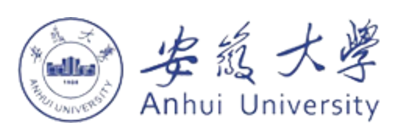
\includegraphics[width=.5\textwidth]{pic/logo-ahu}
  \bicaption{测试图片\\第二行题注}{Test Pic\\Sec Row}
  \label{fig:logo}
\end{figure}
\centerline{-----------$\uparrow$-----------Space Check-----------$\uparrow$-----------}

我们在这儿插入一行字;

我们在这儿再插入一行字;

我们在这儿插入一行字;

我们在这儿再插入一行字;

我们在这儿插入一行字;

我们在这儿再插入一行字;

我们在这儿插入一行字;

我们在这儿再插入一行字;

\section{数学环境}

\subsection{数学符号}

模板定义了一些正体(upright)的数学符号:
\begin{center}
  \begin{tabular}{rl}
    \toprule
    符号                 & 命令 \\
    \midrule
    常数$\eu$     & \verb|\eu| \\
    复数单位$\iu$ & \verb|\iu| \\
    微分符号$\diff$ & \verb|\diff| \\
    $\argmax$         & \verb|\argmax| \\
    $\argmin$         & \verb|\argmin| \\
    \bottomrule
  \end{tabular}
\end{center}

更多的例子:
\begin{equation}
\eu^{\iu\pi} + 1 = 0
\end{equation}
\begin{equation}
\frac{\diff^2u}{\diff t^2} = \int f(x) \diff x
\end{equation}
\begin{equation}
\argmin_x f(x)
\end{equation}

\subsection{定理、引理和证明}

\begin{definition}
  If the integral of function $f$ is measurable and non-negative, we define
  its (extended) \textbf{Lebesgue integral} by
  \begin{equation}
  \int f = \sup_g \int g,
  \end{equation}
  where the supremum is taken over all measurable functions $g$ such that
  $0 \leq g \leq f$, and where $g$ is bounded and supported on a set of
  finite measure.
\end{definition}

\begin{example}
  Simple examples of functions on $\mathbf{R}^d$ that are integrable
  (or non-integrable) are given by
  \begin{equation}
  f_a(x) =
  \begin{cases}
  |x|^{-a} & \text{if } |x| \leq 1,\\
  0 & \text{if } x > 1.
  \end{cases}
  \end{equation}
  \begin{equation}
  F_a(x) = \frac{1}{1 + |x|^a}, \qquad \text{all } x \in \mathbf{R}^d.
  \end{equation}
  Then $f_a$ is integrable exactly when $a < d$, while $F_a$ is integrable
  exactly when $a > d$.
\end{example}

\begin{lemma}[Fatou]
  Suppose $\{f_n\}$ is a sequence of measurable functions with $f_n \geq 0$.
  If $\lim_{n \to \infty} f_n(x) = f(x)$ for a.e. $x$, then
  \begin{equation}
  \int f \leq \liminf_{n \to \infty} \int f_n.
  \end{equation}
\end{lemma}

\begin{remark}
  We do not exclude the cases $\int f = \infty$,
  or $\liminf_{n \to \infty} f_n = \infty$.
\end{remark}

\begin{corollary}
  Suppose $f$ is a non-negative measurable function, and $\{f_n\}$ a sequence
  of non-negative measurable functions with
  $f_n(x) \leq f(x)$ and $f_n(x) \to f(x)$ for almost every $x$. Then
  \begin{equation}
  \lim_{n \to \infty} \int f_n = \int f.
  \end{equation}
\end{corollary}

\begin{proposition}
  Suppose $f$ is integrable on $\mathbf{R}^d$. Then for every $\epsilon > 0$:
  \begin{enumerate}
    \renewcommand{\theenumi}{\roman{enumi}}
    \item There exists a set of finite measure $B$ (a ball, for example) such that
    \begin{equation}
    \int_{B^c} |f| < \epsilon.
    \end{equation}
    \item There is a $\delta > 0$ such that
    \begin{equation}
    \int_E |f| < \epsilon \qquad \text{whenever } m(E) < \delta.
    \end{equation}
  \end{enumerate}
\end{proposition}

\begin{theorem}
  Suppose $\{f_n\}$ is a sequence of measurable functions such that
  $f_n(x) \to f(x)$ a.e. $x$, as $n$ tends to infinity.
  If $|f_n(x)| \leq g(x)$, where $g$ is integrable, then
  \begin{equation}
  \int |f_n - f| \to 0 \qquad \text{as } n \to \infty,
  \end{equation}
  and consequently
  \begin{equation}
  \int f_n \to \int f \qquad \text{as } n \to \infty.
  \end{equation}
\end{theorem}

\begin{proof}
  Trivial.
\end{proof}



\subsection{自定义}

\newtheorem*{axiomofchoice}{Axiom of choice}
\begin{axiomofchoice}
  Suppose $E$ is a set and ${E_\alpha}$ is a collection of
  non-empty subsets of $E$. Then there is a function $\alpha
  \mapsto x_\alpha$ (a ``choice function'') such that
  \begin{equation}
  x_\alpha \in E_\alpha,\qquad \text{for all }\alpha.
  \end{equation}
\end{axiomofchoice}

\newtheorem{observation}{Observation}[chapter]
\begin{observation}
  Suppose a partially ordered set $P$ has the property
  that every chain has an upper bound in $P$. Then the
  set $P$ contains at least one maximal element.
\end{observation}
\begin{proof}[A concise proof]
  Obvious.
\end{proof}

\newtheorem{observationvar2}[observation]{Observationvar2}
\begin{observationvar2}
  Suppose a partially ordered set $P$ has the property
  that every chain has an upper bound in $P$. Then the
  set $P$ contains at least one maximal element.
\end{observationvar2}
\begin{proof}[A concise proof]
  Obvious.
\end{proof}

我们在这儿插入一行字;

我们在这儿再插入一行字;

我们在这儿插入一行字;

我们在这儿再插入一行字;

我们在这儿插入一行字;

我们在这儿再插入一行字;

我们在这儿插入一行字;

我们在这儿再插入一行字;

我们在这儿插入一行字;

我们在这儿再插入一行字;

我们在这儿插入一行字;

我们在这儿再插入一行字;

我们在这儿插入一行字;

我们在这儿再插入一行字;

我们在这儿插入一行字;

我们在这儿再插入一行字;

我们在这儿插入一行字;

我们在这儿再插入一行字;

\section{代码环境}
代码环境使用宏包\href{https://mirrors.sustech.edu.cn/CTAN/macros/latex/contrib/listings/listings.pdf}{listings},代码格式设置用命令\verb|\lstset{}|,详细参数设置请参考用户手册。

\begin{lstlisting}[caption1=搜索,caption2=search,label=listsearch]
int binarysearch(const int *arr, int l, int r, int x)
{
    int mid = l + (r - l) / 2;

    while (arr[mid] != x)
    {
        if (r <= l || r < 0)
        return -1;
|\label{line-9}|
        if (arr[mid] > x)
            // If element is smaller than middle
            r = mid - 1;
        else
            // Else element is in right subarray
            l = mid + 1;

        mid = l + (r - l) / 2;
    }
    // When element is not present in array
    return mid;
}
\end{lstlisting}

如代码列表\ref{listsearch}在第\ref{line-9}行出现了跨页,另起一页情况下,可在跨页代码处使用环境逃逸,即使用命令:\verb|\Suppressnumber|,\verb|\Reactivatenumber|。

例如,代码列表\ref{listmerge}在第\ref{merge-line14}行跨页,使用环境逃逸命令的结果:
\begin{lstlisting}[caption1=合并,caption2=merge,label=listmerge]
void merge(int *a, int l, int r, int n)
{
    int *b = (int *)malloc(n * sizeof(int)); /* dynamic memory must be freed */
    int c = l;
    int p1, p2;
    p1 = l;
    p2 = ((l + r) / 2) + 1;
    while ((p1 < ((l + r) / 2) + 1) && (p2 < r + 1))
    {
        if (a[p1] <= a[p2])
        {
            b[c++] = a[p1];
            p1++;
        }|\label{merge-line14}||\Suppressnumber|
\end{lstlisting}
\begin{lstlisting}[firstnumber=last,stepnumber=1]
|\hfill|$(\text{续代码列表}\ref{listmerge})$|\Reactivatenumber|
        else
        {
            b[c++] = a[p2];
            p2++;
        }
    }
    if (p2 == r + 1)
    {
        while ((p1 < ((l + r) / 2) + 1))
        {
            b[c++] = a[p1];
            p1++;
        }
    }
    else
    {
        while ((p2 < r + 1))
        {
            b[c++] = a[p2];
            p2++;
        }
    }

    for (c = l; c < r + 1; c++) a[c] = b[c];

    free(b);
}
\end{lstlisting}
详细代码,可见文件sample.tex。

% 背景知识
\chapter{机动战士介绍}
{\LARGE Fighter。。。}

% 主体章节
\chapter{正文}
正文是学位论文的核心部分,占主要篇幅。

由于研究工作涉及的学科、选题、研究方法、工作进程、结果表达方式的不同,正文可以包括如下相关内容:调查对象、实验和观测方法、仪器设备、材料原料、实验和观测结果、计算方法和编程原理、数据资料、经过加工整理的图表、形成的论点和导出的结论等。总之,作者应根据研究工作的内容,阐明研究方案和实验方法,突出自己的创新性和特色工作,做到论点明确、论据充分、结论可信,与同类和相关工作的比较分析清楚。

正文应该结构合理,层次分明,推理严密,文笔流畅,内容集中简练,图表、参考文献规范。博士学位论文一般为6-10万字,硕士学位论文一般为3-5万字。

% 实验
\chapter{实验}
{\LARGE 1999年的战斗经验。。。}

\renewcommand{\chaptermark}[1]{\markboth{#1}{}}
% 总结
\chapter{总结与展望}
学位论文的总结单独作为一章,但不加章号。

结论是整篇学位论文的总结,是整篇论文的归宿,不是正文中各章节的小结的简单重复。要求精炼、准确、完整地阐述自己的创造性工作或新的见解及其意义和作用。在结论或讨论中可提出尚待解决的问题,进一步研究的设想,仪器设备的改进以及其它与论文工作有关的建议等。

如果不可能导出应有的结论,也可以没有结论而进行必要的讨论。

% 参考文献
% 2015版国标GBT7714-2015
% 2005版国标GBT7714-2005
\Bib{bst/GBT7714-2015}{reference}

% 附录
\appendix
附录是作为论文主体的补充项目,并不是必需的。下列内容可以作为附录编于论文后:
\begin{enumerate}
    \item [(1)] 为了整篇论文材料的完整,但编入正文又有损于编排的条理和逻辑性,这一材料包括比正文更为详尽的信息、研究方法和技术更深入的叙述,建议可以阅读的参考文献题录,对了解正文内容有用的补充信息等。
    \item [(2)] 由于篇幅过大或取材于复制品而不便于编入正文的材料。
    \item [(3)] 不便于编入正文的罕见的珍贵资料或需要特别保密的技术细节和详细方案(这种情况可单列成册)。
    \item [(4)] 对一般读者并非必要阅读,但对本专业同行有参考价值的资料。
    \item [(5)] 某些重要的原始数据、过长的数学推导、计算程序、框图、结构图、注释、统计表、计算机打印输出文件等。
\end{enumerate}

% 攻读学位期间成果
\achievement
\begin{enumerate}[leftmargin=0.7cm]
\renewcommand{\labelenumi}{[\theenumi]}
\item 在读期间的战斗成果
\end{enumerate}

% 致谢
\acknowledgments
谢谢家人,谢谢老师,谢谢朋友,更感谢自己

{\hfill 某年月日}

\end{document} 